\documentclass[aspectratio=169]{beamer}
\geometry{paperwidth=160mm,paperheight=100mm}
\usepackage{beamerthemesidebar}
\usepackage{hyperref}
\usepackage{color}
\usepackage{multimedia}
\usepackage{colortbl}
\usepackage{amsmath}
\usepackage{empheq}
\usepackage{cancel}
\usepackage{amssymb}
\usepackage{amsfonts}
\usepackage{lipsum}
\usepackage{tcolorbox}
\usepackage{tabularx}
\usepackage{caption}
\usepackage{bm}

\setbeamersize{sidebar width right=0pt}
\setbeamertemplate{footline}[frame number]
%
\definecolor{orange}{RGB}{250,167,12}
\definecolor{yellow}{RGB}{246,250,12}
\definecolor{green}{RGB}{128,238,1}
\definecolor{black}{RGB}{0,0,0}
\definecolor{blue}{RGB}{0,0,255}
\definecolor{red}{RGB}{255,0,0}
\definecolor{sepia}{RGB}{94,38,18}
\newcommand{\ve}[1]{{\rm\bf {#1}}}
\newcommand{\q}[1]{\textcolor{blue}{#1}}
\newcommand{\blue}[1]{\textcolor{blue}{#1}}
\newcommand{\sepia}[1]{\textcolor{sepia}{#1}}
\newcommand{\red}[1]{\textcolor{red}{#1}}
\newcommand{\green}[1]{\textcolor{green}{#1}}
\newcommand{\yellow}[1]{\textcolor{yellow}{#1}}
\newcommand{\orange}[1]{\textcolor{orange}{#1}}
\definecolor{burlywood}{RGB}{255,211,155}
\definecolor{chocolate}{RGB}{255,127,36}
\definecolor{tan}{RGB}{210,180,140}
%
\def\onethird{{\textstyle{1\over3}}}
\def\twothirds{{\textstyle{2\over3}}}
\def\fourthirds{{\textstyle{4\over3}}}
\def\onehalf{{\textstyle{1\over2}}}
\def\threehalfs{{\textstyle{3\over2}}}
%
\newcommand{\pd}{\partial}
\newcommand{\aMLT}{\alpha_{\rm MLT}}
\newcommand{\Fconv}{F_{\rm conv}}
\newcommand{\Frad}{F_{\rm rad}}
\newcommand{\Ftot}{F_{\rm tot}}
\newcommand{\Hp}{H_p}
\newcommand{\prad}{p_{\rm rad}}
\newcommand{\pgas}{p_{\rm gas}}
\newcommand{\TTc}{T_{\rm c}}
\newcommand{\rhoc}{\rho_{\rm c}}
\newcommand{\Teff}{T_{\rm eff}}
\newcommand{\Fstar}{F_\star}
\newcommand{\pstar}{p_\star}
\newcommand{\Pstar}{P_\star}
\newcommand{\Rstar}{R_\star}
\newcommand{\rhostar}{\rho_\star}
\newcommand{\Tstar}{T_\star}
%
\title{Theoretical Astrophysics I: Physics of Sun and Stars\\
Lecture 13: Quiz!!!}
\author{\texorpdfstring{\sepia{Petri K\"{a}pyl\"{a} Ivan Mili\'{c}}\newline\blue{\url{pkapyla, milic@leibniz-kis.de}}}{}}
\institute{Institut f\"ur Sonnenphysik - KIS, Freiburg}
\date{\today}
%
\begin{document}
\frame{\titlepage}


%
\frame{
\frametitle{What are we doing today?}
\begin{itemize}
\item This will be a set of short questions, numerical problems, theoretical / conceptual questions to test what you remembered and help you prepare for the exam.
\item You can expect that the problems at the exam will be somewhat more specific. 
\end{itemize}
}
%
%
\frame{
\frametitle{Question 1:}
If a star is in hydrostatic equilibrium, what two forces are in balance? Derive the appropriate expression.
}
%
%
\frame{
\frametitle{Question 2:}
\begin{minipage}{0.54\linewidth}
On the given HR diagram, mark the stars that belong to the main sequence, red giants and white dwarves. 
\end{minipage}
\begin{minipage}{0.45\linewidth}
\begin{figure}
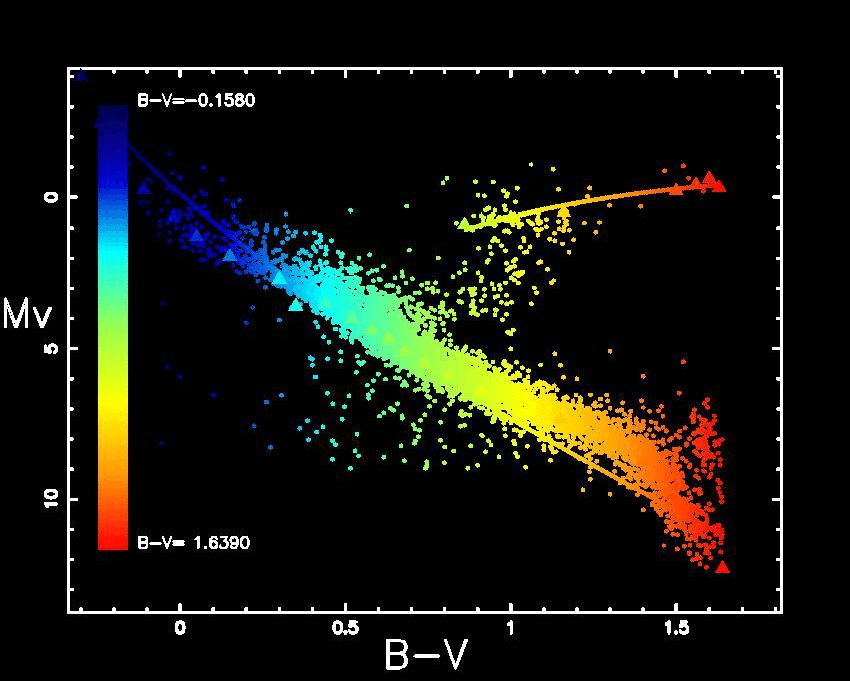
\includegraphics[width=6cm]{figures/hr.png}
\end{figure}
\end{minipage}
}
%
\frame{
\frametitle{Question 3:}
If a blue giant and a red giant star have the same absolute brigthness, and blue giant has effective temperature of 20\,000\,K, while the red giant has effective temperature of 3\,000\,K - how do their radii relate?
}
%
\frame{
\frametitle{Question 4:}
Write down the equation of state (relationship between pressure, density and temperature) for a gas that only consists of Hydrogen and Helium and is: a) completely ionized; b) completely neutral
}
%
\end{document}
% 

